\begin{table}[h!]
\centering
\caption{Detalhamento do modelo obtido com a arquitetura Inception-V3 para a abordagem B.}
\label{tab:shufflenet}
\begin{tabular}{cccccc}
\toprule
\textbf{Otimizador} & \textbf{\emph{Patience}}  & \textbf{Função de Ativação} & \textbf{Acurácia} & \textbf{F-Score} & \textbf{EER} \\
\midrule
RMSprop & 5 & ELU & $0.8394$ & $0.8070$ & $16.9493$ \\
\bottomrule
\end{tabular}
\end{table}

\begin{figure}[H]
\centering
\caption{Histórico de \emph{loss} e acurácia durante o treinamento do modelo obtido com a arquitetura Inception-V3.}
\label{fig:treinamento-inception}
\subfloat[\emph{Loss} durante treinamento da rede Inception-V3 para a abordagem B.\label{subfig:inception-b-loss}]{%
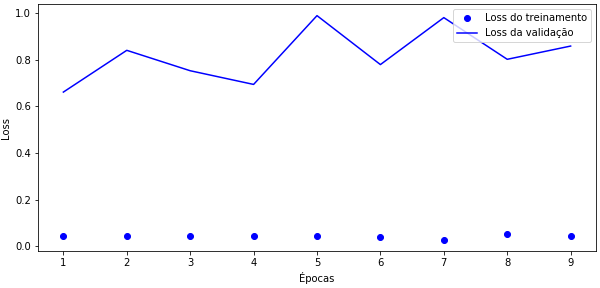
\includegraphics[width=0.47\textwidth]{imgs/inception-b-loss}
}
\hfill
\subfloat[Acurácia durante treinamento da rede Inception-V3 para a abordagem B.\label{subfig:inception-b-acc}]{%
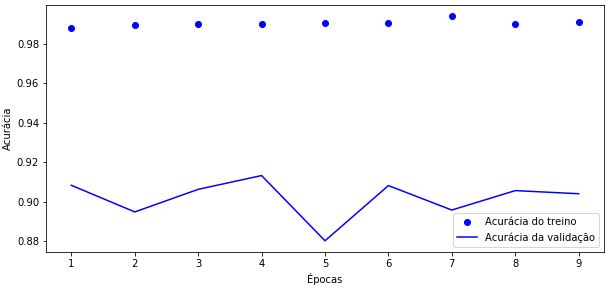
\includegraphics[width=0.47\textwidth]{imgs/inception-b-acc}
}
\end{figure}

\begin{figure}[h]
    \centering
    \caption{Matriz de confusão do modelo obtido com a arquitetura Inception-V3.}\label{fig:matrizes-inception}
    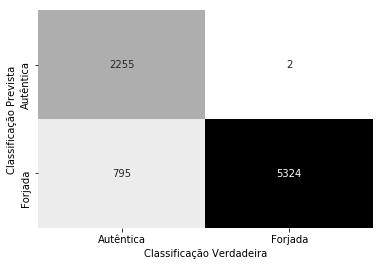
\includegraphics[width=0.6\textwidth]{imgs/matriz-squeezenet-a}
\end{figure}